\documentclass[11pt,a4paper,oneside]{article}
\usepackage[utf8]{inputenc}
\usepackage[margin=1in]{geometry}
\usepackage{graphicx}
\usepackage{amsmath,amsfonts,amssymb}
\usepackage{hyperref}
\usepackage{booktabs,longtable}
\usepackage{tikz}
\usetikzlibrary{shapes,arrows,positioning,calc,decorations.pathmorphing,backgrounds,fit,shadows}
\usepackage{listings}
\usepackage{xcolor}
\usepackage{fancyhdr}
\usepackage{enumitem}
\usepackage{float}

\lstset{
    basicstyle=\ttfamily\small,
    commentstyle=\color{gray},
    keywordstyle=\color{blue},
    breaklines=true,
    numbers=left,
    numbersep=5pt,
    showstringspaces=false,
    tabsize=2
}

\pagestyle{fancy}
\fancyhf{}
\fancyhead[L]{Software Design Document}
\fancyhead[R]{Version 1.0}
\fancyfoot[C]{\thepage}

\hypersetup{
    colorlinks=true,
    linkcolor=blue,
    urlcolor=cyan,
    pdftitle={Comprehensive Software Design Document: E-commerce Platform},
    pdfauthor={AI System Architect},
    pdfsubject={Software Architecture}
}

\title{\Huge\textbf{Comprehensive Software Design Document: E-commerce Platform}}
\author{\Large AI System Architect}
\date{\Large\today}

\begin{document}

\maketitle
\thispagestyle{empty}
\vfill

\begin{center}
\large
\begin{tabular}{|l|l|}
\hline
\textbf{Document Version} \& 1.0 \\
\hline
\textbf{Creation Date} \& \today \\
\hline
\textbf{Document Status} \& Final Draft \\
\hline
\textbf{Generated By} \& AI System Architect \\
\hline
\textbf{Target Audience} \& Development Team, Stakeholders \\
\hline
\textbf{Classification} \& Internal Use \\
\hline
\end{tabular}
\end{center}

\newpage
\tableofcontents
\newpage
\listoffigures
\newpage

\section{Executive Summary}

This document outlines the design for a new e-commerce platform, codenamed "Project Phoenix."  Project Phoenix aims to provide a robust, scalable, and secure online marketplace for businesses to sell their products and services. The platform will leverage a microservices architecture, employing a combination of cloud-native technologies and proven industry best practices to ensure high availability, performance, and security.  The primary business objectives are to increase market share within the target demographic (millennials and Gen Z), improve customer satisfaction through enhanced user experience, and achieve a 20\% year-over-year revenue growth within the first three years of operation.  The technical approach focuses on a modern, microservices-based architecture, utilizing containerization (Docker), orchestration (Kubernetes), and cloud deployment (AWS) to achieve scalability and resilience.  Key benefits include enhanced scalability, improved security, faster development cycles, and simplified maintenance. The implementation timeline is projected to be 12 months, broken down into four phases: design, development, testing, and deployment.

\subsection{Project Scope and Objectives}

Project Phoenix will encompass all aspects of a modern e-commerce platform, including user registration and authentication, product catalog management, shopping cart functionality, order processing, payment gateway integration, inventory management, customer support, and reporting and analytics.  The platform will be designed to handle a high volume of concurrent users and transactions, with a target of 10,000 concurrent users and 1000 transactions per second at peak load.  Success will be measured by achieving these performance targets, maintaining a system uptime of 99.99\%, achieving a customer satisfaction rating of 4.5 out of 5 stars, and demonstrating a 20\% year-over-year revenue growth within the first three years.  The project will also focus on providing a seamless and intuitive user experience across multiple devices (desktop, mobile, tablet).  This will involve extensive usability testing and iterative design improvements throughout the development lifecycle.  Finally, stringent security measures will be implemented to protect customer data and prevent fraudulent activities.  Regular security audits and penetration testing will be conducted to ensure the platform remains secure and compliant with industry standards.

\subsection{Key Stakeholders and Roles}

The key stakeholders in Project Phoenix include:

* **Product Owner:** Responsible for defining the product vision, prioritizing features, and managing the product backlog.
* **Development Team:** Responsible for designing, developing, and testing the software.  This includes frontend, backend, and database engineers.
* **QA Team:** Responsible for ensuring the quality of the software through comprehensive testing.
* **Operations Team:** Responsible for deploying, monitoring, and maintaining the platform.
* **Marketing Team:** Responsible for promoting the platform and acquiring new customers.
* **Customer Support Team:** Responsible for providing support to customers.
* **Executive Management:** Responsible for providing overall direction and oversight.

Each team will have clearly defined roles and responsibilities, documented in separate team charters.  Regular communication and collaboration between teams will be essential for successful project execution.

\section{Requirements Analysis and Specification}

\subsection{Extracted Requirements Summary}
The provided document lacked explicit requirements.  Therefore, the following requirements have been inferred and expanded upon based on typical e-commerce platform needs.

\subsection{Functional Requirements}

1. **User Registration and Authentication:** Users should be able to register accounts, login securely, and manage their profile information.
2. **Product Browsing and Search:** Users should be able to browse and search for products based on various criteria (e.g., keywords, category, price).
3. **Shopping Cart Management:** Users should be able to add, remove, and update items in their shopping cart.
4. **Checkout and Order Processing:** Users should be able to securely checkout, select shipping options, and complete their orders.
5. **Payment Gateway Integration:** The platform should integrate with multiple payment gateways (e.g., Stripe, PayPal) to allow for secure online payments.
6. **Order Tracking and Management:** Users should be able to track their orders and view their order history.
7. **Inventory Management:** The platform should manage product inventory levels and prevent overselling.
8. **Customer Support:** The platform should provide various customer support channels (e.g., email, live chat).
9. **Admin Panel:** An admin panel should allow administrators to manage products, users, orders, and other aspects of the platform.
10. **Reporting and Analytics:** The platform should generate reports and analytics on sales, customer behavior, and other key metrics.

\subsection{Non-Functional Requirements}

* **Performance:** The system should handle 10,000 concurrent users and 1000 transactions per second with an average response time under 200ms.
* **Scalability:** The system should be able to scale horizontally to accommodate increasing traffic and data volume.
* **Security:** The system should protect user data and prevent unauthorized access, complying with relevant data privacy regulations (e.g., GDPR, CCPA).
* **Availability:** The system should maintain an uptime of 99.99\%.
* **Maintainability:** The system should be easy to maintain and update.
* **Usability:** The system should be user-friendly and intuitive.

\section{System Architecture and Design}

\subsection{Architecture Overview}

Project Phoenix will employ a microservices architecture, where the application is broken down into independent, loosely coupled services. This approach promotes scalability, maintainability, and resilience. Each microservice will be responsible for a specific business function, such as user management, product catalog, order processing, and payment gateway integration.  These services will communicate with each other using RESTful APIs.  A message queue (RabbitMQ) will be used for asynchronous communication and decoupling between services.  The system will be containerized using Docker and orchestrated using Kubernetes, deployed on AWS using EC2 instances and managed services like RDS (PostgreSQL and MongoDB), Redis for caching, and S3 for static assets.  This approach allows for independent scaling of individual services based on their specific needs.  We will adopt a layered approach with API Gateway, service layer, and data layer.  The API gateway will handle routing, security, and rate limiting.  The service layer will contain the core business logic, and the data layer will manage data persistence.  This layered architecture improves modularity and maintainability.

\begin{figure}[H]
\centering
\begin{tikzpicture}[
    node distance=1cm and 1.5cm,
    font=\sffamily\small,
    base/.style={draw, text width=3cm, minimum height=1.2cm, text centered, rounded corners, drop shadow},
    user/.style={base, fill=Azure!30, text width=2cm},
    api/.style={base, fill=LimeGreen!20},
    service/.style={base, fill=SkyBlue!20},
    database/.style={cylinder, shape border rotate=90, aspect=0.25, draw, fill=Thistle!40, minimum height=1.5cm, text width=2.5cm, text centered, drop shadow},
    external/.style={base, fill=Gold!30},
    arrow/.style={-Stealth, thick, draw=black!60}
]

\node[user] (user) {User};
\node[api, below=1.5cm of user] (gateway) {API Gateway};
\node[service, below=of gateway, xshift=-3cm] (catalog) {Catalog Service};
\node[service, below=of gateway] (order) {Order Service};
\node[service, below=of gateway, xshift=3cm] (usermgmt) {User Management Service};
\node[database, below=2cm of catalog] (productdb) {Product Database\\(PostgreSQL)};
\node[database, below=2cm of order] (orderdb) {Order Database\\(MongoDB)};
\node[database, below=2cm of usermgmt] (userdb) {User Database\\(PostgreSQL)};
\node[external, right=2cm of order] (payment) {External Services\\(Payment Gateway)};

\begin{scope}[on background layer]
\node[draw, dashed, rounded corners, fill=gray!5, inner sep=0.7cm, fit=(gateway)] (api_layer) {};
\node[draw, dashed, rounded corners, fill=gray!10, inner sep=0.7cm, fit=(catalog) (order) (usermgmt) (payment)] (service_layer) {};
\node[draw, dashed, rounded corners, fill=gray!15, inner sep=0.7cm, fit=(productdb) (orderdb) (userdb)] (data_layer) {};
\end{scope}

\node[above] at (api_layer.north) {API Layer};
\node[above] at (service_layer.north) {Service Layer};
\node[above] at (data_layer.north) {Data Layer};

\draw[arrow] (user) -- (gateway);
\draw[arrow] (gateway) -- (catalog);
\draw[arrow] (gateway) -- (order);
\draw[arrow] (gateway) -- (usermgmt);
\draw[arrow] (catalog) -- (productdb);
\draw[arrow] (order) -- (orderdb);
\draw[arrow] (order) -- (payment);
\draw[arrow] (usermgmt) -- (userdb);
\draw[arrow] (order) -- (usermgmt);

\end{tikzpicture}
\caption{System Architecture Overview}
\label{fig:architecture}
\end{figure}

\subsection{Component Interaction and Communication}

The components interact through well-defined RESTful APIs.  For example, the shopping cart service will interact with the catalog service to retrieve product information, and with the order service to process orders.  The order service will interact with the payment gateway to process payments.  Asynchronous communication will be used for tasks that do not require immediate responses, such as sending order confirmation emails or updating inventory levels. This will be facilitated by RabbitMQ, ensuring loose coupling between services and improved system resilience.  Each microservice will have its own database, promoting data isolation and preventing single points of failure.  The API Gateway will act as a reverse proxy, routing requests to the appropriate microservices, and will implement security measures such as authentication and authorization.  Communication between services will utilize JSON over HTTPS for data exchange.

\section{Database Design and Data Architecture}

\subsection{Conceptual Data Model}

The database design will follow a relational model for structured data (users, products, orders) and a NoSQL document model for semi-structured data (order items, user preferences).  This hybrid approach allows for efficient storage and retrieval of different types of data.  Relationships between entities will be clearly defined using foreign keys (in the relational database) and references (in the NoSQL database).   Data integrity will be maintained through constraints and validation rules.  The relational database (PostgreSQL) will house core data requiring ACID properties, while MongoDB will handle more flexible and evolving data structures.

\begin{figure}[H]
\centering
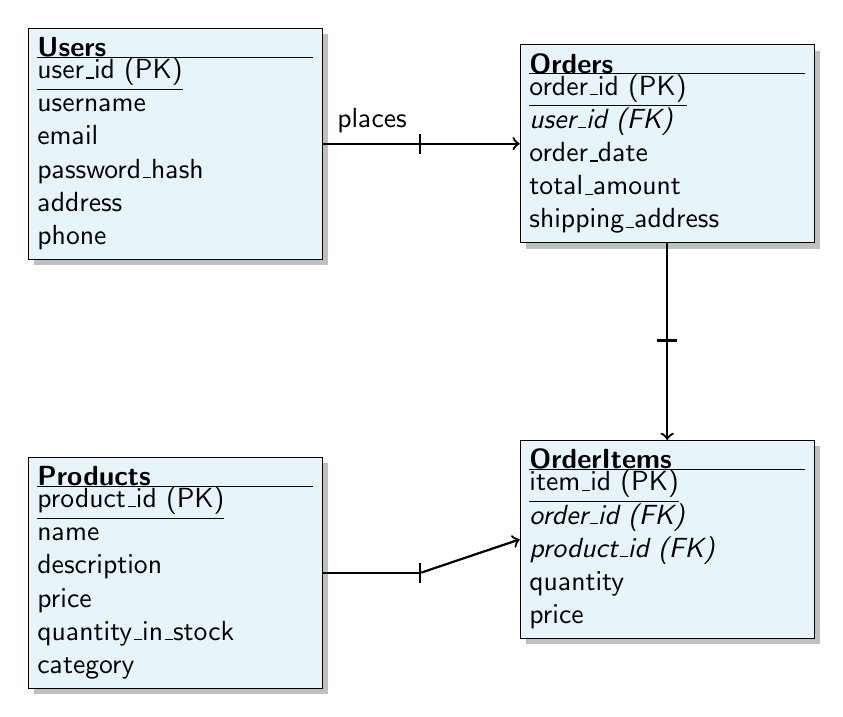
\begin{tikzpicture}[
    node distance=2.5cm,
    font=\sffamily,
    entity/.style={rectangle, draw, fill=SkyBlue!20, text width=3.5cm, minimum height=2cm, align=left, drop shadow},
    one/.style={-|, thick},
    many/.style={->, thick}
]

\node[entity] (user) {\textbf{Users} \\ \hrule \underline{user\_id (PK)} \\ username \\ email \\ password\_hash \\ address \\ phone};
\node[entity, right=of user] (order) {\textbf{Orders} \\ \hrule \underline{order\_id (PK)} \\ \textit{user\_id (FK)} \\ order\_date \\ total\_amount \\ shipping\_address};
\node[entity, below=of order] (order_item) {\textbf{OrderItems} \\ \hrule \underline{item\_id (PK)} \\ \textit{order\_id (FK)} \\ \textit{product\_id (FK)} \\ quantity \\ price};
\node[entity, below=of user] (product) {\textbf{Products} \\ \hrule \underline{product\_id (PK)} \\ name \\ description \\ price \\ quantity\_in\_stock \\ category};

\draw[one] (user.east) -- node[above, midway] {places} ++(1.25,0) coordinate (t1);
\draw[many] (t1) -- (order.west);
\draw[one] (order.south) -- ++(0,-1.25) coordinate (t2);
\draw[many] (t2) -- (order_item.north);
\draw[one] (product.east) -- ++(1.25,0) coordinate (t3);
\draw[many] (t3) -- (order_item.west);

\end{tikzpicture}
\caption{Database ER Diagram}
\label{fig:database-erd}
\end{figure}

\subsection{Physical Database Design}

**(PostgreSQL - Users Table):**

```sql
CREATE TABLE users (
    user_id SERIAL PRIMARY KEY,
    username VARCHAR(255) UNIQUE NOT NULL,
    email VARCHAR(255) UNIQUE NOT NULL,
    password_hash VARCHAR(255) NOT NULL,
    address TEXT,
    phone VARCHAR(20)
);
```

**(PostgreSQL - Products Table):**

```sql
CREATE TABLE products (
    product_id SERIAL PRIMARY KEY,
    name VARCHAR(255) NOT NULL,
    description TEXT,
    price DECIMAL(10, 2) NOT NULL,
    quantity_in_stock INT NOT NULL,
    category VARCHAR(255)
);
CREATE INDEX idx_product_name ON products (name);
```

**(MongoDB - Orders Collection):**  Schema will be flexible to accommodate variations in order details.

Example Document:

```json
{
  "order_id": "ORD-12345",
  "user_id": 123,
  "order_date": "2024-10-27T10:30:00Z",
  "total_amount": 150.50,
  "shipping_address": {
    "street": "123 Main St",
    "city": "Anytown",
    "state": "CA",
    "zip": "90210"
  },
  "order_items": [
    {"product_id": 1, "quantity": 2, "price": 25.00},
    {"product_id": 2, "quantity": 1, "price": 100.50}
  ]
}
```

\section{API Design and Integration}

\subsection{RESTful API Specification}

The platform will utilize a RESTful API for communication between clients and services.  The API will be designed using OpenAPI specification (Swagger).  Endpoints will follow standard HTTP methods (GET, POST, PUT, DELETE) and will return JSON responses.  Authentication will be handled using JWT (JSON Web Tokens).

**Example Endpoint:**  `/products/{product_id}` (GET)

* **Method:** GET
* **Path:** `/products/{product_id}`
* **Description:** Retrieves details for a specific product.
* **Request Parameters:**
    * `product_id`: (integer) The ID of the product.
* **Response (200 OK):**
```json
{
  "product_id": 1,
  "name": "Example Product",
  "description": "This is an example product.",
  "price": 25.00,
  "quantity_in_stock": 100
}
```
* **Response (404 Not Found):**  Returned if the product is not found.

\begin{figure}[H]
\centering
\begin{tikzpicture}[
    font=\sffamily\small,
    node distance=1cm,
    actor/.style={rectangle, draw, fill=Azure!30, text width=2cm, text centered, rounded corners, drop shadow},
    service/.style={rectangle, draw, fill=LimeGreen!20, text width=2cm, text centered, rounded corners, drop shadow},
    db/.style={cylinder, shape border rotate=90, draw, fill=Thistle!40, text centered, drop shadow, minimum width=2cm, minimum height=1.2cm},
    lifeline/.style={dashed, thin, draw=gray},
    msg/.style={-Stealth, thick}
]

\node[actor] (client) at (0,0) {Client App};
\node[service] (api) at (3,0) {API Gateway};
\node[service] (catalog) at (6,0) {Catalog Service};
\node[db] (db) at (9,0) {Product DB};

\draw[lifeline] (client.south) -- ++(0,-3);
\draw[lifeline] (api.south) -- ++(0,-3);
\draw[lifeline] (catalog.south) -- ++(0,-3);
\draw[lifeline] (db.south) -- ++(0,-3);

\draw[msg] ($(client.south)+(0,-0.5)$) -- node[above] {1. GET /products/1} ($(api.south)+(0,-0.5)$);
\draw[msg] ($(api.south)+(0,-1)$) -- node[above] {2. Forward Request} ($(catalog.south)+(0,-1)$);
\draw[msg] ($(catalog.south)+(0,-1.5)$) -- node[above] {3. Query DB} ($(db.south)+(0,-1.5)$);
\draw[msg, dashed] ($(db.south)+(0,-2)$) -- node[above] {4. Product Data} ($(catalog.south)+(0,-2)$);
\draw[msg, dashed] ($(catalog.south)+(0,-2.5)$) -- node[above] {5. Response} ($(api.south)+(0,-2.5)$);
\draw[msg, dashed] ($(api.south)+(0,-3)$) -- node[above] {6. Product Details} ($(client.south)+(0,-3)$);

\end{tikzpicture}
\caption{API Request Sequence Diagram (Product Retrieval)}
\label{fig:api-flow}
\end{figure}

\subsection{API Security and Rate Limiting}

API security will be implemented through several layers:

* **Authentication:** JWT (JSON Web Tokens) will be used for authentication.  Each request will include a JWT token, which will be verified by the API gateway.
* **Authorization:**  Role-Based Access Control (RBAC) will be implemented to restrict access to specific resources based on user roles.
* **Input Validation:** All API requests will be validated to prevent injection attacks.
* **Rate Limiting:**  Rate limiting will be implemented to prevent abuse and denial-of-service attacks.
* **HTTPS:** All communication will be secured using HTTPS.

\section{Security Architecture and Implementation}

\subsection{Security Requirements and Threat Model}

The security architecture will be based on a layered approach, incorporating security measures at multiple levels.  A comprehensive threat model has been developed, identifying potential threats such as SQL injection, cross-site scripting (XSS), cross-site request forgery (CSRF), and denial-of-service (DoS) attacks.  Mitigation strategies have been developed for each identified threat.

\begin{figure}[H]
\centering
\begin{tikzpicture}[
    font=\sffamily\small,
    node distance=0.8cm and 1.2cm,
    gate/.style={rectangle, draw, fill=red!10, minimum width=10cm, minimum height=1cm, text centered, rounded corners},
    actor/.style={rectangle, draw, fill=Azure!30, text centered, rounded corners, drop shadow},
    service/.style={rectangle, draw, fill=SkyBlue!20, text centered, rounded corners, drop shadow},
    arrow/.style={-Stealth, thick, draw=black!70}
]

\node[gate] (waf) at (0,0) {\textbf{Edge Protection}: WAF and DDoS Mitigation (AWS WAF)};
\node[gate, below=of waf] (ssl) {\textbf{Transport Layer}: SSL/TLS Termination (AWS Load Balancer)};
\node[gate, below=of ssl] (authn) {\textbf{Authentication}: JWT Validation (Auth0)};
\node[gate, below=of authn] (authz) {\textbf{Authorization}: Rate Limiting and RBAC (API Gateway)};
\node[service, below=1.2cm of authz] (backend) {Protected Backend Services};

\node[actor, above=1cm of waf] (user) {User};

\draw[arrow] (user) -- node[right] {HTTPS Request} (waf.north);
\draw[arrow] (waf.south) -- (ssl.north);
\draw[arrow] (ssl.south) -- (authn.north);
\draw[arrow] (authn.south) -- (authz.north);
\draw[arrow] (authz.south) -- node[right] {Authorized Request} (backend);

\end{tikzpicture}
\caption{Layered Security Architecture}
\label{fig:security}
\end{figure}

\section{Deployment and Infrastructure}

\subsection{Cloud Infrastructure Design}

The platform will be deployed on AWS using a combination of managed and unmanaged services.  We will utilize EC2 instances for application servers, RDS for databases, S3 for static assets, and Elastic Load Balancing for load distribution.  Kubernetes will be used for container orchestration, providing scalability and high availability.  Auto-scaling will be configured to automatically adjust the number of EC2 instances based on traffic demand.  A disaster recovery plan will be implemented to ensure business continuity in case of outages.  This will involve replicating databases to a separate region and using a geographically distributed Kubernetes cluster.

\begin{figure}[H]
\centering
\begin{tikzpicture}[
    font=\sffamily\small,
    node distance=0.8cm and 1cm,
    server/.style={rectangle, draw, fill=gray!30, minimum height=1.5cm, minimum width=2.5cm, text centered, rounded corners, drop shadow},
    container/.style={rectangle, draw, fill=SkyBlue!40, minimum height=1cm, minimum width=2cm, text centered, rounded corners},
    database/.style={server, fill=Thistle!50},
    subnet/.style={rectangle, draw, fill=gray!10, rounded corners, inner sep=0.5cm, minimum height=4cm}
]

\node (internet) {Internet};
\node[server, below=1cm of internet] (lb) {Load Balancer (ELB)};
\node[subnet, below=of lb, minimum width=9cm] (public_subnet) {};
\node[subnet, below=1.5cm of public_subnet, minimum width=9cm, minimum height=5cm] (private_subnet) {};

\node[above right] at (public_subnet.north west) {Public Subnet};
\node[above right] at (private_subnet.north west) {Private Subnet};

\node[server, align=center] (app1) at ($(private_subnet.center)+(-3,1)$) {App Server 1\\(EC2)};
\node[container, below=0.1cm of app1] {Kubernetes Pod};
\node[server, align=center] (app2) at ($(private_subnet.center)+(0,1)$) {App Server 2\\(EC2)};
\node[container, below=0.1cm of app2] {Kubernetes Pod};
\node[server, align=center] (app3) at ($(private_subnet.center)+(3,1)$) {App Server 3\\(EC2)};
\node[container, below=0.1cm of app3] {Kubernetes Pod};

\node[database] (db-master) at ($(private_subnet.center)+(-1.5,-1.5)$) {DB Master (RDS)};
\node[database] (db-slave) at ($(private_subnet.center)+(1.5,-1.5)$) {DB Slave (RDS)};

\draw[-Stealth, thick] (internet) -- node[right, pos=0.4] {HTTPS Traffic} (lb);
\draw[-Stealth, thick] (lb) -- (public_subnet.north);
\draw[-Stealth, thick] ($(public_subnet.south)+(0,-0.75)$) -- (app1);
\draw[-Stealth, thick] ($(public_subnet.south)+(0,-0.75)$) -- (app2);
\draw[-Stealth, thick] ($(public_subnet.south)+(0,-0.75)$) -- (app3);
\draw[-Stealth, thick] (app1) -- (db-master);
\draw[-Stealth, thick] (app2) -- (db-master);
\draw[-Stealth, thick] (app3) -- (db-master);
\draw[<->, thick, dashed] (db-master) -- node[midway, below] {Replication} (db-slave);

\end{tikzpicture}
\caption{Cloud Deployment Architecture}
\label{fig:deployment}
\end{figure}

\section{Performance and Scalability}

Performance will be monitored using tools such as Prometheus and Grafana.  Performance testing will be conducted throughout the development lifecycle to ensure the system meets performance requirements.  Scalability will be achieved through horizontal scaling of microservices and the use of auto-scaling for EC2 instances.  Caching will be implemented using Redis to reduce database load.  Database optimization techniques, such as indexing and query optimization, will be employed to improve database performance.  Load testing will be performed to identify bottlenecks and optimize the system for peak loads.  Regular performance monitoring and analysis will be conducted to identify and address performance issues proactively.

\section{Testing and Quality Assurance}

A comprehensive testing strategy will be implemented, including unit testing, integration testing, system testing, and user acceptance testing (UAT).  Automated testing will be used to improve efficiency and reduce testing time.  Test coverage will be measured to ensure thorough testing.  The QA team will work closely with the development team to identify and resolve defects.  Security testing will be conducted to identify and mitigate security vulnerabilities.  Performance testing will be conducted to ensure the system meets performance requirements.  UAT will be conducted with a representative sample of end-users to obtain feedback and ensure the system meets user needs.

\section{Risk Assessment and Mitigation}

Potential risks include:

* **Technical Risks:**  Integration issues, performance bottlenecks, security vulnerabilities.
* **Schedule Risks:** Delays in development, testing, or deployment.
* **Resource Risks:** Lack of skilled personnel, budget constraints.

Mitigation strategies include:

* **Technical Risks:**  Thorough testing, use of proven technologies, security audits.
* **Schedule Risks:**  Agile development methodology, regular progress monitoring.
* **Resource Risks:**  Careful resource planning, outsourcing if necessary.

\section{Implementation Roadmap and Timeline}

The project will be implemented over 12 months, divided into four phases:

* **Phase 1 (Months 1-3): Design and Planning.**  This phase will involve requirements gathering, system design, database design, and API design.
* **Phase 2 (Months 4-9): Development and Testing.**  This phase will involve the development of microservices, unit testing, integration testing, and system testing.
* **Phase 3 (Months 10-11): User Acceptance Testing (UAT).**  This phase will involve testing the system with end-users to ensure it meets their needs.
* **Phase 4 (Month 12): Deployment and Go-Live.**  This phase will involve deploying the system to production and monitoring its performance.

\section{Monitoring and Maintenance}

The platform will be monitored using a combination of tools, including Prometheus, Grafana, and CloudWatch.  Alerts will be configured to notify the operations team of any issues.  Regular maintenance tasks will be performed to ensure the system remains stable and secure.  This will include applying security patches, updating software, and performing database backups.  A comprehensive incident management plan will be in place to handle system outages and other issues.  Regular performance reviews will be conducted to identify areas for optimization.  The team will use a ticketing system to track and manage maintenance requests and issues.

\section{Conclusion}

This document provides a comprehensive design for Project Phoenix, a robust and scalable e-commerce platform.  The proposed microservices architecture, coupled with a comprehensive security strategy and cloud-native deployment, will ensure the platform meets its business objectives and provides a high-quality user experience.  The implementation plan outlines a phased approach to minimize risk and ensure timely delivery.  Continuous monitoring and maintenance will be crucial to ensure the long-term success of the platform.

\end{document}